% This work is licensed under the Creative Commons
% Attribution-NonCommercial 3.0 Unported License. To view a copy of this
% license, visit http://creativecommons.org/licenses/by-nc/3.0/.

% This work is licensed under the Creative Commons
% Attribution-NonCommercial 3.0 Unported License. To view a copy of this
% license, visit http://creativecommons.org/licenses/by-nc/3.0/.

% ==========================================================================
%                     Festlegung der Dokumentenklasse
% ==========================================================================

% Dokumentklasse für Aufsätze, Berichte, etc.
\documentclass[paper=a4, german, titlepage]{scrartcl}

% Behebt ein paar Fehler in Latex
\usepackage{fixltx2e}

% ==========================================================================
%                            Detailtypographie
% ==========================================================================

\usepackage{microtype}

% ==========================================================================
%                             Zeichenkodierung
% ==========================================================================

% UTF-8 als Eingabe-Kodierung und T1 als Fontkodierung
\usepackage[utf8]{inputenc}
\usepackage[T1]{fontenc}

% ==========================================================================
%                               Schriftarten
% ==========================================================================

\usepackage{lmodern}

% ==========================================================================
%                           Spracheinstellungen
% ==========================================================================

% Deutsche Zeichenketten und deutsche Namen für die Referenzobjeke
\usepackage[german]{babel, varioref}

% ==========================================================================
%                  Aufzählungen, Referenzen und Links
% ==========================================================================

\usepackage{enumitem}

% Verlinkungen innerhalb und außerhalb des PDF-Dokuments
\usepackage{hyperref}

% Formattiert URLs, so dass sie sich z.B. besser vom Text abheben
\usepackage{url}

% TrueType-Schrift für URLs		
% \urlstyle{tt}		

% ==========================================================================
%                        Bibliograhphie und Anhang
% ==========================================================================

\newcommand{\theappendix}{
  \clearpage
  \appendix
}

% Deutsche Guillemets mit \enquote{}
\usepackage[german=guillemets]{csquotes}

\usepackage[style=numeric-comp, backend=biber]{biblatex}
\bibliography{../literatur.bib}

% Nachnamen in Kapitälchen
\renewcommand*{\mkbibnamelast}[1]{\textsc{#1}}

% ==========================================================================
%                    Grafiken, Abbildungen und Tabellen
% ==========================================================================

% Verwenden von Farben und Grafiken
\usepackage{graphicx}
\usepackage{xcolor}

% Einbinden von ganzen PDF-Seiten
\usepackage{pdfpages}

% kleine Schrift für Bildunterschriften, Fettgedruckte Bildunterschriften
\usepackage[font=small,	labelfont=bf, format=plain]{caption}

% Für mehrere Objekte nebeneinander mit eigenen Bildunterschriften
\usepackage{subcaption}

% Beinhaltet \FloatBarrier , sodass nach diesem Befehl keine Floats mehr erscheinen
\usepackage{placeins}

% Text umläuft Fließobjekte
%\usepackage{wrapfig}

% Tabellensatz
% \usepackage{tabularx}
\usepackage{booktabs}
\usepackage{longtable}

% Zum Verdrehen von Objekten. Nur mäßig verwenden.
% \usepackage{rotating}

% Setzen des Pfades für eingebundene Bilder
% \graphicspath{{figs/}{bilder/}}

% ==========================================================================
%                    Mathematikumgebungen und Einheiten
% ==========================================================================

% Paket für mathematische Umgebungen und Funktionen
\usepackage[intlimits]{amsmath}

% Zusätzliche Mathematische Schriftarten
\usepackage{amsfonts}

% Zusätzliche Mathematische Symbole
\usepackage{amssymb}

% Zum Setzen Kommutativer Diagramme
% \usepackage{amscd}

% Textsatz in der Matheumgebung
\usepackage{amstext}

% Aufrechte griechische Buchstaben
%\usepackage{upgreek}


% Diagramme mit tikz und Gnuplot zeichnen
% \usepackage{tikz}
% \usepackage{tikz-qtree}
% \usepackage{gnuplot-lua-tikz}

% ==========================================================================
%               automatischer Satz von Einheiten mit SIUnitX
% ==========================================================================

\usepackage[
% Stellt den Fehler separat dar: Siehe SIUnitX-Manual
  separate-uncertainty = true,
]{siunitx}

% Babel stellt SIUnitX auf deutsch ein, wenn german gewählt wird
\addto\extrasgerman{\sisetup{locale = DE}}

% Kürzen von Einheiten in SIUnitX ermöglichen
% \usepackage{cancel}


% ==========================================================================
%                            Textsatzparameter
% ==========================================================================

% Vermeidung von "Schusterjungen" Höchstwert 10000, dann dürfen
% theoretisch keine Schusterjungen mehr auftreten.
\clubpenalty = 3000
% Vermeidkung von "Hurenkindern" Höchstwert 10000, dann dürfen
% theoretisch keine Hurenkinder mehr auftreten.  Es werden beide
% Einstellungen benötigt.
\widowpenalty = 3000
\displaywidowpenalty = 3000


\newcommand{\name}[1]{\textsc{#1}}
\newcommand{\pdn}[3]{%
\ensuremath{\frac{\partial^{#1} #2}{\partial #3^{#1}}}}
\newcommand{\pd}[2]{%
\ensuremath{\frac{\partial #1}{\partial #2}}}
\renewcommand{\d}{\ensuremath{\mathrm{d}}}
\newcommand{\iunt}{\ensuremath{\mathrm{i}}} % imaginary unit

\titlehead{{TU Dortmund \hfill WS~13/14\\}
Fakultät Physik\\ Fortgeschrittenenpraktikum}

\subject{Versuchsprotokoll}
\title{Signale auf Leitungen}
\subtitle{Versuch 52}

\author{Daniel Meißner\\
{\normalsize\url{daniel.meissner@udo.edu}}
\and
Kevin Moch\\
{\normalsize\url{kevin.moch@udo.edu}}}

\date{21. Februar 2014}

\begin{document}
\maketitle

\tableofcontents
\clearpage

\section{Einleitung}

In diesem Versuch soll das Verhalten von elektrischen Signalen in 
Leitungen, insbesondere in Koaxialkabeln, untersucht werden.
Dabei werden sowohl leitungsspezifische Konstanten bestimmt, 
als auch zeitliche Verläufe von Signalen beobachtet.
\FloatBarrier

\section{Theorie}

\begin{figure}
\centering
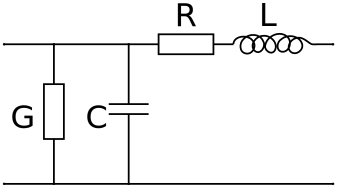
\includegraphics[scale=0.6]{ersatzschaltung}
\label{fig:ersatz}
\caption{%
Ersatzschaltung eines Koaxialkabels zwischen $x$ und $x + \d x$.
Die Größen $R, L, G, C$ heißen Leitungskonstanten oder
Leitungsbeläge.  Bei einer verlustfreien Leitung ist $R = G = 0$.
Durch eine Betrachtung dieser Ersatzschaltung kann die
Telegraphengleichung hergeleitet werden.}
\end{figure}

Die Beschreibung der Ausbreitung von Signalen auf Leitungen ist
Gegenstand der Leitungstheorie.  Eine Leitung (zum Beispiel eine
Koaxialleitung, die in diesem Versuch verwendet wird) kann durch zwei
parallel verlaufende Leiter modelliert werden.  Grundaufgabe der
Leitungstheorie ist es, den zeitlichen Verlauf von Stromstärke $I(t, x)$
und Spannung $U(t, x)$ an jedem Ort $x$ der Leitung zu bestimmen.

Dazu wird ein Leitungstück von $x$ nach $x + \d x$ durch die
Ersatzschaltung aus Abbildung~\ref{fig:ersatz} dargestellt.  Die
Leitungsbeläge $R, L, G, C$ heißen auch Leitungskonstanten: $L$
und $C$ heißen Induktivitäts- bzw. Kapazitätsbelag, $R$ und $G$
heißen ohmscher Belag bzw. Querleitfähigkeitsbelag.  Die beiden
letzten kommen durch die endliche Leitfähigkeit des
Leitermaterials (Längsspannungsverluste) und dielektrische
Verlustströme zwischen der Isolierung der beiden Leiter zustande.

\subsection{Telegraphengleichung}

Im allgemeinen ergibt sich durch Betrachtung der Ersatzschaltung
ein System gekoppelter partieller Differentialgln. für $U$ und
$I$.  Im Falle konstanter Beläge kann dieses entkoppelt werden
und es folgt eine verallgemeinerte Wellengleichung:
%
\begin{equation}
\label{eq:wellengl.}
\pdn{2}{U}{x} - LC \pdn{2}{U}{t} = (LG+RC) \pd{U}{t} + RGU
\end{equation}
%
Diese Gleichung wird auch oft als Telegraphengleichung
bezeichnet.  Die Lösungen sind gedämpfte, hin- und rücklaufende
harmonische Wellen:
%
\begin{equation}
\label{eq:loesung}
U(t, x) = U_0 \,e^{\iunt\omega t \pm \gamma x}
\end{equation}
%
Der Faktor $\gamma = \alpha + \iunt \beta
= \sqrt{(R+\iunt \omega L)(G + \iunt \omega C)}$ heißt
Ausbreitungskonstante, $\alpha$ heißt Dämpfungsbelag und $\beta$
heißt Phasenbelag.  Die Phasengeschwindigkeit der Welle ist daher
frequenzabhängig und führt zu einer Verzerrung des Signals.

\subsection{Leitungswellenwiderstand}

Die Art der Verzerrung wird vom Leitungswellenwiderstand
beeinflußt, welcher durch das Verhältnis von Strom- und
Spannungswellen, die sich in eine gemeinsame Richtung ausbreiten,
bestimmt ist.  Für ein sinusförmiges Signal mit der Frequenz
$\omega$ ist der Wellenwiderstand daher
%
\begin{equation}
\label{eq:wellenwiderstand}
Z_0 = \frac{U(\omega)}{I(\omega)} = \sqrt{\frac{R + \iunt \omega
L}{G + \iunt \omega C}}\:.
\end{equation}
%

\subsection{Spannungs- und Strompulse}

In der Digital- und Nachrichtentechnik haben die Signale, die
über eine Leitung übertragen werden, oft die Form eines Pulses.
Die Lösungen der entsprechenden Telegraphengleichung haben dann
die Form eines hin- und rücklaufenden Pulses, der durch die
Reflexion am Leitungsende entsteht.  Der Quotient
%
\begin{equation}
\Gamma = \frac{U_\text{r}}{U_0} = \frac{Z_\text{L} - Z_0}{Z_\text{L} + Z_0}
\end{equation}
%
heißt Reflexionsfaktor, wobei $Z_L$ hier die Lastimpedanz am Verbraucher
darstellt.  Mit seiner Hilfe kann die Form der rücklaufenden Welle aus
dem Eingangspuls berechnet werden.  Dazu wird
die \name{Laplace}-Transformation verwendet.  Sei nämlich
$\tilde{U}_0(s)$ die \name{Laplace}-Transformierte der Spannung des
einlaufenden und $\tilde{U}_\text{r}(s)$
die \name{Laplace}-Transformierte der Spannung des reflektierten Signals
am Ort $x$ zur Zeit $t$, dann gilt
%
\begin{equation}
\label{eq:reflex}
\tilde{U}_\text{r}(s) = \Gamma\, \tilde{U}_0(s).
\end{equation}
%
Aus der Umkehrung dieser Formel unter Ausnutzung der
inversen \name{Laplace}-Transformation der zeitliche Verlauf der
Spannung $U_\text{r}(t, x)$ bestimmt werden.  Je nach
Leitungsabschluß ergeben sich hier verschiedene Signalformen.  Im
Fall $Z_\text{L} = Z_0$ liegt die sogenannte Leitungsanpassung vor,
d.\,h. der Reflexionsfaktor $\Gamma = 0$ und es gibt keine
reflektierte Welle.

\subsection{Ausgewählte Leitungsabschlüsse}
In diesem Abschnitt werden die Signalverläufe zu drei verschiedenen
Abschlußwiderständen berechnet.  Die erhaltenen Funktionen werden später
verwendet, um eine Ausgleichsrechnung mit den aufgenommenen Meßwerten
durchzuführen.  Der einlaufende Signalverlauf\footnote{Die Amplitude
wird hier auf 1 normiert, um die Rechnungen nicht zu überladen.  Da
die \name{Laplace}-Transformation eine lineare Abbildung ist, kann ein
Faktor für die Amplitude nachträglich hinzugefügt werden.}
kann mit der \name{Heaviside}-Funktion~$\Theta$ so geschrieben werden:
%
\begin{equation}
U_0(t) = \Theta(t).
\end{equation}
%
Die \name{Laplace}-Transformierte lautet dann $\tilde{U}_0(s) = s^{-1}$.
Mit Formel~\eqref{eq:reflex} wird daraus der Reflex am Leitungsende
berechnet.

\paragraph{Abschluß durch Induktivität}  Im Falle einer Induktivität als
Abschluß ist $Z_\text{L} = \iunt\omega L$  und damit ergibt sich für $s
= \iunt\omega$ der Reflexionsfaktor zu
%
\begin{equation}
\Gamma = \frac{sL - Z_0}{sL + Z_0} = \frac{s - \tau^{-1}}{s + \tau^{-1}}
\end{equation}
%
mit $\tau := L/Z_0$. Jetzt wird gemäß Formel~\eqref{eq:reflex} das
reflektierte Signal berechnet.  Zerlege dazu $\Gamma \tilde{U}_0(s)$ in
Partialbrüche:
%
\begin{equation}
\tilde{U}_\text{r}(s) = \Gamma\tilde{U}_0(s) = \frac{s - \tau^{-1}}{s(s
+ \tau^{-1})} = \frac{2}{s + \tau^{-1}} - \frac{1}{s}
\end{equation}
%
Nach den Eigenschaften der \name{Laplace}-Transformation bezüglich
Translation das reflektierte Signal für $t>0$ erhalten:
%
\begin{equation}
\label{eq:ind_reflex}
U_\text{r}(t) = 2e^{-\frac{t}{\tau}} - 1.
\end{equation}

\paragraph{Abschluß durch Induktivität und ohmschen Widerstand}  In
diesem Fall wird $Z_\text{L} = R + \iunt \omega L$ und der
Reflexionsfaktor lautet 
%
\begin{equation}
\Gamma = \frac{R + sL - Z_0}{R + sL - Z_0} = \frac{s + (R-Z_0)L^{-1}}{s + \tau^{-1}}
\end{equation}
%
mit $\tau := L/(Z_0 + R)$.  Jetzt wird analog zu oben verfahren.  Eine
Partialbruchzerlegung von $\Gamma \tilde{U}_0(s)$ liefert:
%
\begin{equation}
\tilde{U}_\text{r} (s) = \Gamma \tilde{U}_0(s) = \frac{s + (R -
Z_0)L^{-1}}{s(s + \tau^{-1})} = \frac{\Gamma_0}{s} + \frac{1
- \Gamma_0}{s + \tau^{-1}}
\end{equation}
%
mit $\Gamma_0 := \frac{R - Z_0}{R + Z_0}$.  Daraus wird das reflektierte
Signal durch Rücktransformation erhalten:
%
\begin{equation}
\label{eq:ind_ohm_reflex}
U_\text{r}(t) = \Gamma_0 + (1 - \Gamma_0) e^{-\frac{t}{\tau}}.
\end{equation}

\paragraph{Abschluß durch Kapazität und ohmschen Widerstand}  Hier ist
$Z_\text{L} = R + \frac{1}{\iunt \omega C}$ und der Reflexionsfaktor
lautet dann:
%
\begin{equation}
\Gamma = \frac{\frac{1}{sC} + R - Z_0}{\frac{1}{sC} + R + Z_0}
= \frac{\Gamma_0 s + \tau^{-1}}{s + \tau^{-1}} 
\end{equation}
%
mit $\Gamma_0$ wie oben und $\tau := (R+Z_0) C$.  Nach der
Partialbruchzerlegung
%
\begin{equation}
\Gamma \tilde{U}_0(s) = \frac{1}{s} + \frac{\Gamma_0 - 1}{s + \tau^{-1}}
\end{equation}
%
lautet nach Rücktransformation das reflektierte Signal so:
%
\begin{equation}
\label{eq:cap_ohm_reflex}
U_\text{r}(t) = 1 + (\Gamma_0 - 1) e^{-\frac{t}{\tau}}.
\end{equation}

\subsection{Mehrfachreflexionen}

\section{Versuchsaufbau und Durchführung}

Zum Versuch werden verschiedene Meßgeräte, einige Abschlußwiderstände
und die zu untersuchenden Koaxialkabel selbst benötigt.  Dazu stehen
vier verschiedene Koaxialkabel zur Verfügung.  Jeder Versuchsabschnitt
ist im wesentlichen aus drei Komponenten aufgebaut: Meßgerät,
Signalgenerator und zu messendes Kabel.

\subsection{Bestimmung der Kabellänge}

Um die Länge eines Kabels zu bestimmen, wird ein Spannungspuls auf das
Kabel gegeben und dann mithilfe eines Oszilloskops die Zeitdifferenz
zwischen einlaufendem und reflektiertem Signal bestimmt.  Da sich das
Signal innerhalb der Leitung mit der Ausbreitungsgeschwindigkeit $c =
c_0/\sqrt{\epsilon_\text{r}}$ bewegt, gilt für die Länge des Kabels
daher:
%
\begin{equation}
\label{eq:laenge}
L = c \frac{\Delta t}{2} = \frac{c_0 \Delta t}{2 \sqrt{\epsilon_r}}.
\end{equation}

\subsection{Bestimmung der Leitungskonstanten}

Zur Bestimmung der Leitungskonstanten wird das zu vermessene Kabel an
das RLC-Meßgerät angeschlossen, welches automatisch die Art des
Abschlußwiderstands erkennt und die entsprechenden Impedanzen anzeigt.

\subsection{Bestimmung der Dämpfung}

Zur Bestimmung der Dämpfung wird ein Rechteckpuls durch ein kurzes Kabel
an einen Spektrumsanalysator geschickt und dort mithilfe
einer \textit{Fast Fourier Transform} spektral analysiert.  Für das
kurze Kabel wird keine Dämpfung angenommen und die Amplituden der ersten
Oberwellen werden notiert.

Für ein zweites längeres Kabel wird dieselbe Prozedur durchgeführt und
die so erhaltenen Amplituden mit denjenigen, die mit kurzen Kabel
erhalten worden sind, verglichen.

\subsection{Mehrfachreflexion}

\subsection{Untersuchung der Abschlußwiderstände}

% This work is licensed under the Creative Commons
% Attribution-NonCommercial 3.0 Unported License. To view a copy of this
% license, visit http://creativecommons.org/licenses/by-nc/3.0/.

\section{Auswertung}

Aus den gewonnenen Daten, die nachfolgend vorgestellt werden, kann man
den Elastizitätsmodul der untersuchten Metalle und Legierungen
errechnen. Um eine lineare Regression\footnote{benutzt wurde hierfür die
  \texttt{ipython}-Umgebung mit der \texttt{numpy}-Bibliothek in der
  Version 1.6.2} anwenden zu können, stellt man die Zusammenhänge
\eqref{eq:durchbiegung-einseitig} und \eqref{eq:durchbiegung-beidseitig}
so dar:
%
\begin{align}
  \label{eq:lineare-durchbiegung-einseitig}
  D(x) &= f(Lx^2-\frac{x^3}{3}) & f(u) &:= \frac{F}{2EI}u
\end{align}
Dies ist für die einseitige Aufhängung des Stabes. Für die beidseitige
Aufhängung ergibt sich:
\begin{align}
  \label{eq:lineare-durchbiegung-beidseitig}
  D(x) &= \begin{cases}
    g(3L^2x-4x^3) & 0\le x\le \frac{L}{2}\\
    g(4x^3-12Lx^2 + 9L^2x - L^3) & \frac{L}{2}\le x\le L
  \end{cases}
  & g(u) &:= \frac{F}{48EI}u
\end{align}
%
Hier können nun die Größen $A_g = F/(48EI)$ und $A_f = F/(2EI)$ bestimmt
werden. Umstellen von der beiden Größen nach $E$ liefert:
\begin{align}
  \label{eq:e-modul}
  E &= \frac{F}{2A_fI} & E =& \frac{F}{48A_gI}
\end{align}
Da diese fehlerbehaftet sind, wird eine \name{Gauß}-Fehlerfortpflanzung
durchgeführt:
%
\begin{equation}
  \label{eq:gaussfehler-f}
  \Delta E = \sqrt{\left(\frac{\partial E}{\partial A_f}
      \cdot\Delta A_f\right)^2}
  = \frac{F\cdot\Delta A_f}{2A_f^2I}
\end{equation}
%
\begin{equation}
  \label{eq:gaussfehler-g}
  \Delta E = \sqrt{\left(\frac{\partial E}{\partial A_g}\cdot\Delta
      A_g\right)^2}
  = \frac{F\cdot\Delta A_g}{48A^2_gI}
\end{equation}

Zur Bestimmung des Fehlers, der beim Messen des Durchmessers gemacht
wird, wird die Formel für die Standardabweichung benutzt:

\begin{equation}
  \label{eq:durchmesser-fehler}
  \sqrt{\frac{1}{n-1} \sum_{i=1}^n (d_i - \bar{d})^2}
\end{equation}

Die Flächenträgheitsmomente werden wie folgt berechnet. Für den
Stahlstab mit kreisförmigem Querschnitt $Q = \{(r\cos\phi, r\sin\phi) :
0\le r\le \frac{d}{2}, 0\le\phi\le2\pi\}$ gilt:
\[
I = \int_Q y^2\:\d(x, y)
\]
Durch Anwendung der Transformation $T\colon M\to Q, (r, \phi) \mapsto
(r\cos\phi, r\sin\phi)$ mit $M = \{(r,\phi) : 0\le r\le d/2,
0\le\phi\le2\pi\}$ ergibt sich:
\[
I = \int_Q y^2\:\d(x, y) = \int_M r^3\sin^2\phi\:\d(r, \phi) =
\int_{r=0}^\frac{d}{2} r^3 \int_{\phi=0}^{2\pi} \sin^2\phi\:\d\phi\,\d r
= \frac{d^4\pi}{64}
\]

Das Flächenträgheitsmoment für die beiden Stäbe mit quadratischem
Querschnitt $Q = \{(x, y) : 0\le x\le d, 0\le y\le d\}$ (Aluminium und
Messing) ergibt sich so:
\[
\int_Q y^2\:\d(x, y) = \int_{y=0}^d\int_{x=0}^d y^2\:\d x\,\d y =
d\int_0^d y^2\:\d y = \frac{d^4}{3}
\]

\subsection{Bestimmung des Elastizitätsmoduls von Stahl}

Die gemessenen Durchbiegung in Abhängigkeit vom Ort können in der
Tabelle~\ref{tab:stahl} nachgesehen werden. Es wurden immer die
Durchbiegungen $D_v(x)$ ohne Gewicht und die Durchbiegungen $D_n(x)$ mit
Gewicht bestimmt. Die eingespannte Länge ist $L=\SI{49.5}{\centi\metre}$
und als Gewicht haben wir die Masse $m=\SI{1680.9}{\gram}$
verwendet. Gemäß Formel~\eqref{eq:echte_durchbiegung} errechnet sich die
effektive Durchbiegung~$D(x)$, die Grundlage für weitere Berechnungen
ist.

Die Stichprobe zur Bestimmung des Durchmessers $d$ findet man in
Tabelle~\ref{tab:stahl-durchmesser}. Nach der Bestimmung des
arithmetischen Mittels und der Standardabweichung
(Formel~\eqref{eq:durchmesser-fehler}) ergibt sich für den Durchmesser:
%
\begin{equation}
  d = \SI{9.985(3)}{\milli\meter}
\end{equation}
%
Abbildung~\ref{fig:stahl} zeigt eine Darstellung der Meßwerte und der
Regressionsgerade. Die roten Punkte wurden für die Regression
herangezogen. Daraus erhält man diese Gleichung:
%
\begin{equation}
  D(x) = \SI{0.016}{\per\cubic\metre} 
  \left(Lx^2 - \frac{x^3}{3}\right)  - \SI{0.001}{\metre}
\end{equation}
%
Der Fehler für die Steigung ergibt sich aus der Regression zu:
%
\begin{equation}
  \Delta A_f = \SI{0.0008}{\per\cubic\metre}
\end{equation}
%
Mithilfe der Steigung $A_f$ und Formel~\eqref{eq:e-modul} und nach der
\name{Gauss}-Fehlerfortpflanzung in Formel~\eqref{eq:gaussfehler-f} erhält man
folgenden Wert für $E$:
%
\begin{equation}
  \label{eq:wert-stahl-emodul}
  E = \SI{1078(53)}{\kilo\newton\per\milli\metre\squared}
\end{equation}
%

\begin{table}
  \centering\small
  \begin{tabular}{SSS}
    \toprule
    {$x/\si{\centi\metre}$} &
    {$D_v/\si{\micro\metre}$} &
    {$D_n/\si{\micro\metre}$} \\
    \midrule
    2.7 &    550 &    510 \\
    5.0 &    600 &    470 \\
    9.0 &    600 &    220 \\
    13.0 &    590 &    185 \\
    17.0 &    540 &    136 \\
    21.0 &    530 &    280 \\
    25.0 &    460 &    312 \\
    27.0 &    430 &    377 \\
    32.0 &    310 &    475 \\
    35.0 &    200 &    490 \\
    38.0 &    170 &    544 \\
    40.0 &    198 &    600 \\
    42.0 &    198 &    647 \\
    44.0 &    195 &    700 \\
    46.0 &    180 &    749 \\
    48.0 &    177 &    795 \\
    \bottomrule
  \end{tabular}
  \caption{Meßwerte zur Durchbiegung des Stahlstabes}
  \label{tab:stahl}
\end{table}

\begin{table}
  \centering\small
  \begin{tabular}{S}
    \toprule
    {$d/\si{\milli\metre}$}\\
    \midrule
    9.986 \\
    9.989 \\
    9.983 \\
    9.988 \\
    9.986 \\
    9.982 \\
    9.982 \\
    9.985 \\
    9.985 \\
    9.981 \\
    \bottomrule
  \end{tabular}
  \caption{Durchmesser des Stahlstabes}
  \label{tab:stahl-durchmesser}
\end{table}

\begin{figure}
  \centering
  \includegraphics[width=0.8\textwidth]{stahl-einseitig-kreisfoermig.pdf}
  \caption{Meßwerte mit linearer Regression für den Stahlstab}
  \label{fig:stahl}
\end{figure}

\subsection{Bestimmung des Elastizitätsmoduls von Aluminium}

Die gemessenen Durchbiegungen für den Aluminiumstab ist in
Tabelle~\ref{tab:aluminium} zu finden. Die Werte zum Durchmesser in
Tabelle~\ref{tab:aluminium-durchmesser}. Die eingespannte Länge beträgt
$L=\SI{49.6}{\centi\metre}$ und als Gewicht haben wir die Masse
$m=\SI{5416}{\gram}$ verwendet. Der Mittelwert des Durchmessers und
seine Standardabweichung~(Formel~\eqref{eq:durchmesser-fehler}) betragen:
%
\begin{equation}
  d = \SI{9.985(3)}{\milli\metre}
\end{equation}
%
Nach der Regression, die in Abbildung~\ref{fig:aluminium} zu sehen ist,
erhält man folgende Gleichung:
%
\begin{equation}
  D(x) = \SI{0.044}{\per\cubic\metre} \left(Lx^2 - \frac{x^3}{3}\right)
\end{equation}
%
Der Fehler für die Steigung ergibt sich aus der Regression zu:
%
\begin{equation}
  \Delta A_f = \SI{0.0004}{\per\cubic\metre}
\end{equation}
%
Wie bereits beim Stahl bestimmt man hieraus mit der Steigung~$A_f$ und
Formel~\eqref{eq:e-modul} den E-Modul und mithilfe der Fehlerrechnung
aus Formel~\eqref{eq:gaussfehler-f} läßt sich folgender Wert angeben:
%
\begin{equation}
  E = \SI{73.0(7)}{\kilo\newton\per\milli\metre\squared}  
\end{equation}

\begin{table}
  \centering\small
  \begin{tabular}{SSS}
    \toprule
    {$x/\si{\centi\metre}$} & 
    {$D_v/\si{\micro\metre}$} & 
    {$D_n/\si{\micro\metre} $} \\
    \midrule
    2.7  &   920   &    930 \\
    7.5  &  1030   &  1170  \\
    12.5 &  1210   &  1550  \\
    17.5 &  1430   &  2060  \\
    22.5 &  1680   &  2680  \\
    27.5 &  2020   &  3410  \\
    30.0 &  2220   &  3800  \\
    32.0 &  2350   &  4150  \\
    34.0 &  2520   &  4480  \\
    36.0 &  2710   &  4850  \\
    38.0 &  2850   &  5230  \\
    40.0 &  3030   &  5610  \\
    42.0 &  3190   &  6000  \\
    44.0 &  3320   &  6410  \\
    46.0 &  3660   &  6770  \\
    48.0 &  3800   &  7240  \\
    \bottomrule
  \end{tabular}
  \caption{Meßwerte zur Durchbiegung des Aluminiumstabes}
  \label{tab:aluminium}
\end{table}

\begin{table}
  \centering\small
  \begin{tabular}{S}
    \toprule
    {$d/\si{\milli\metre}$}\\
    \midrule
    9.984 \\
    9.988 \\
    9.984 \\
    9.971 \\
    9.979 \\
    9.980 \\
    9.994 \\
    9.986 \\
    9.988 \\
    9.982 \\
    \bottomrule
  \end{tabular}
  \caption{Durchmesserx des Aluminiumstabes}
  \label{tab:aluminium-durchmesser}
\end{table}

\begin{figure}
  \centering
  \includegraphics[width=0.8\textwidth]{aluminium-einseitig-quadratisch.pdf}
  \caption{Meßwerte mit linearer Regression für den Aluminiumstab}
  \label{fig:aluminium}
\end{figure}


\subsection{Bestimmung des Elastizitätsmoduls von Messing}

Der Messingstab ist beidseitig auf die Länge $L =
\SI{55.1}{\centi\metre}$ eingespannt. Als Gewicht verwenden wir die
Masse $m = \SI{4.1}{\kilogram}$. Die Bestimmung des Durchmessers liefert
die Tabelle~\ref{tab:messing-durchmesser}. Mittelwert und
Standartabweichung~(Formel~\eqref{eq:durchmesser-fehler}) ergeben sich so:
%
\begin{equation}
  d = \SI{9.983(9)}{\milli\meter}
\end{equation}
%
In Abbildung~\ref{fig:messing} sind die Regressionen
dargestellt. Die beiden Gleichungen lauten folgendermaßen:
%
\begin{align}
  D(x) &= \SI{0.0070}{\per\cubic\metre} 
  ( 3L^2x-4x^3 ) - \SI{0.0002}{\cubic\metre} 
  & 0 \le x \le \frac{L}{2}\\
  D(x) &= \SI{0.0063}{\per\cubic\metre}
  (4x^3 - 12Lx^2 + 9L^2x - L^3) + \SI{0.0001}{\cubic\metre} 
  & \frac{L}{2} \le x \le L
\end{align}
%
Die Fehler für die Steigungen ergeben sich aus der Regression zu:
%
\begin{align}
  \Delta A_f &= \SI{0.0004}{\per\cubic\metre}\\
  \Delta A_g &= \SI{0.0003}{\per\cubic\metre}
\end{align}
%
In Tabelle~\ref{tab:messing} finden sich die Meßwerte dazu. Als
Ergebnis erhält man aus Formel~\eqref{eq:e-modul}, in die man die beiden
Steigungen $A_f$ und $A_g$ einsetzt, zwei Werte für $E$:
\begin{align}
 E&=\SI{143.8(88)}{\kilo\newton\per\milli\metre\squared} &
 E&=\SI{159.4(54)}{\kilo\newton\per\milli\metre\squared}
\end{align}

\begin{figure}
  \centering
  \includegraphics[width=0.8\textwidth]{messing-beidseitig-quadratisch.pdf}
  \caption{Meßwerte mit linearer Regression für den Messingstab}
  \label{fig:messing}
\end{figure}

\begin{table}
  \centering
 
  \begin{tabular}{SSS}
    \toprule
    {$x/\si{\centi\metre}$} & 
    {$D_v/\si{\micro\metre}$} & 
    {$D_n/\si{\micro\metre} $} \\
    \midrule
    3.0 &  1010 &   1040 \\
    8.0 &  1080 &   1310 \\
    13.0&  1170 &   1640 \\
    18.0&  1230 &   1940 \\
    20.0&  1230 &   2040 \\
    22.0&  1250 &   2140 \\
    24.0&  1250 &   2220 \\
    26.0&  1280 &   2280 \\
    31.6&  2880 &   3910 \\
    33.0&  2860 &   3900 \\
    35.0&  2820 &   3810 \\
    37.0&  2770 &   3750 \\
    39.0&  2750 &   3680 \\
    44.0&  2680 &   3370 \\
    49.0&  2620 &   3020 \\
    54.0&  2600 &   2690 \\
    \bottomrule
  \end{tabular}
  \caption{Meßwerte für den Messingstab}
  \label{tab:messing}
\end{table}

\begin{table}
  \centering
  \begin{tabular}{S}
    \toprule
    {$d/\si{\milli\metre}$}\\
    \midrule
    9.979 \\
    9.986 \\
    9.987 \\
    9.975 \\
    9.973 \\
    9.981 \\
    9.983 \\
    9.997 \\
    9.974 \\
    9.998 \\
    \bottomrule
  \end{tabular}
  \caption{Meßwerte für den Durchmesser des Messingstabes}
  \label{tab:messing-durchmesser}
\end{table}


%%% Local Variables: 
%%% mode: latex
%%% TeX-master: "protokoll"
%%% End: 


\end{document}
